\documentclass[../main.tex]{subfiles}
\begin{document}
    \begin{enumerate}[a), font=\bfseries]
        \item Écrire \textbf{deux expression littérale} donnant l'aire du rectangle grisé.
        \begin{center}
            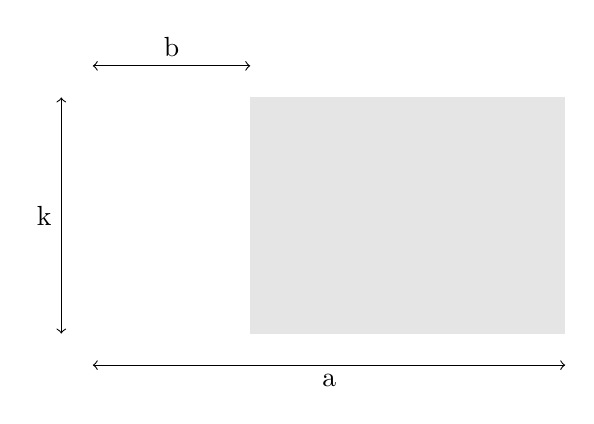
\begin{tikzpicture}
                \def\L{6}
                \def\l{3}
                \def\ll{2}
                \def\x{.4}
                \coordinate(A)at(0,0);
                \coordinate(B)at(\L,0);
                \coordinate(C)at(\L,\l);
                \coordinate(D)at(0,\l);
                \coordinate(E)at(\ll,0);
                \coordinate(F)at(\ll,\l);
                \coordinate(A0)at(-\x,0);
                \coordinate(D0)at(-\x,\l);
                \coordinate(D1)at(0,\l+\x);
                \coordinate(F1)at(\ll,\l+\x);
                \coordinate(A1)at(0,-\x);
                \coordinate(B1)at(\L,-\x);
                \tkzDrawPolygon(A,B,C,D)
                \draw(E)--(F);
                \path(A0)--(D0)node[midway, left]{k};
                \draw[<->](A0)--(D0);
                \path(D1)--(F1)node[midway, sloped, above]{b};
                \draw[<->](D1)--(F1);
                \path(A1)--(B1)node[midway, sloped, below]{a};
                \draw[<->](A1)--(B1);
                \fill[black!10!](E)rectangle(C);
            \end{tikzpicture}
        \end{center}
        \item En vous aidant de la question précédente, compléter la propriété ci dessous:
        \begin{simplebox}
            Pour tout nombre $a$, $b$, $k$: $$k(a-b)=$$
            \vspace{.3cm}
        \end{simplebox}
        \item \textbf{Application :} développer les expression littérales suivantes:
        \begin{center}
            \begin{minipage}{.45\linewidth}
                $3(x-4)=$
            \end{minipage}\hspace{.05\linewidth}
            \begin{minipage}{.45\linewidth}
                $-5\times(2-x)=$
            \end{minipage}
        \end{center}
    \end{enumerate}
\end{document}